\documentclass{article}

\usepackage{booktabs}
\usepackage{setspace}
\usepackage{threeparttable}
\usepackage{rotating}
\usepackage{blindtext}
\usepackage{amsmath}
\usepackage[
    backend=biber,
    style=bwl-FU,
    url=false,
    doi=false,
    eprint=false
]{biblatex}
\addbibresource{first_bib_file.bib}

\author{
  Frutiger, Nils\\
  \texttt{abc.def@ghi.com}
  }

\begin{document}

\ \vspace{1.0cm}
\begin{center}
{\LARGE This is the Title}\\[2.5cm]



\hspace{10cm}\begin{minipage}[h]{12cm}
\begin{tabbing}
Author: \hspace{1.5cm} \= Nils Frutiger \\
Major: \> Banking and Finance  \\
Student number: \> 16-114-472 \\
Date: \> 31.10.2021\\
\end{tabbing}
\end{minipage}
\end{center}


\newpage

\begin{abstract}
\blindtext
\Blindtext


\end{abstract}
\newpage

\section{Text}
\blindtext
\cite{Milgrom}
\newline
\cite{DevenowRationalHerdingInFinancialEconomics}
\Blindtext

\newpage
\section{Table}

This is a table:

\begin{table}[h]
	\centering
	\caption{total non-financial debt as percentage of GDP}
	\begin{tabular}{l|rrr|rr}
		\midrule
		\multicolumn{1}{r}{} & \multicolumn{3}{c|}{Levels} & \multicolumn{2}{c}{Changes} \\
		\cmidrule{2-6}    \multicolumn{1}{r}{} & \multicolumn{1}{c}{2000} & \multicolumn{1}{c}{2010} & \multicolumn{1}{c|}{2019} & \multicolumn{1}{c}{2000-10} & \multicolumn{1}{c}{2010-19} \\
		\midrule
		Switzerland & 241   & 243   & 284   & 2     & 41 \\
		United States & 186   & 250   & 250   & 65    & 0 \\
		Germany & 187   & 199   & 181   & 12    & -18 \\
		Norway & 184   & 270   & 270   & 86    & 0 \\
		France & 197   & 266   & 329   & 69    & 63 \\
		Austria & 196   & 238   & 226   & 42    & -12 \\
		Australia & 154   & 204   & 236   & 50    & 32 \\
		Spain & 173   & 285   & 268   & 112   & -17 \\
		Sweden & 201   & 269   & 289   & 68    & 20 \\
		Japan & 313   & 342   & 380   & 29    & 38 \\
		Italy & 192   & 248   & 258   & 56    & 10 \\
		United Kingdom & 180   & 267   & 275   & 87    & 8 \\
		\midrule
		Advanced Economies\footnotemark[2] & 212   & 254   & 272   & 42    & 18 \\
			\end{tabular}%
	\label{tab:total non financial debt as percentage of GDP}%
\end{table}%

\newpage

\section{figure}
This is a figure:

\begin{figure}[h]
	\centering
	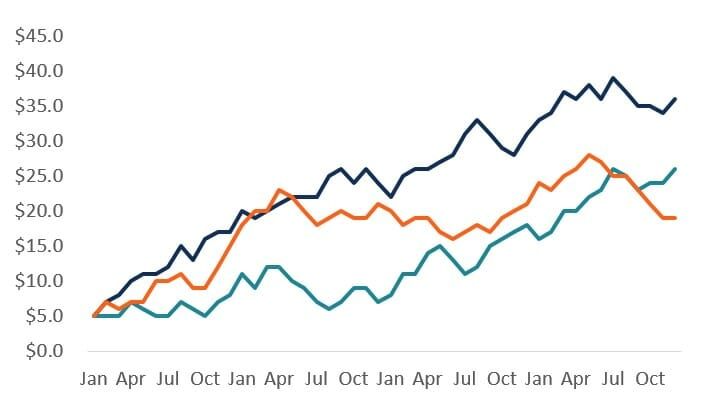
\includegraphics[width=0.9\textwidth]{line-graph.jpg}
	\caption{line graph}
	{Source: Web}
	\label{fig:basicgrowthreg}
\end{figure}



\section{Bibliography}
\printbibliography

\end{document}



